\documentclass{article}
\usepackage[utf8x]{inputenc}
\usepackage{ucs}
\usepackage{amsmath} 
\usepackage{amsfonts}
\usepackage{upgreek}
\usepackage[english,russian]{babel}
\usepackage{graphicx}
\usepackage{float}
\usepackage{textcomp}
\usepackage{hyperref}
\usepackage{geometry}
  \geometry{left=2cm}
  \geometry{right=1.5cm}
  \geometry{top=1cm}
  \geometry{bottom=2cm}
\usepackage{tikz}
\usepackage{ccaption}
\usepackage{multicol}
%\setlength{\columnsep}{1.5cm}
%\setlength{\columnseprule}{0.2pt}


\begin{document}
\pagenumbering{gobble}

\newpage

\subsection*{Арифметика указателей}
Пусть есть одномерный статический массив и указатель на 4-й элемент этого массива:
\begin{verbatim}
int numbers[6] = {4, 8, 15, 16, 23, 42};
int* p = &numbers[3];
\end{verbatim}
Чему равны следующие выражения:
\begin{multicols}{3}
\begin{enumerate}
\item \begin{verbatim} numbers[5] \end{verbatim}
\item \begin{verbatim} *p \end{verbatim}
\item \begin{verbatim} *(p+1) \end{verbatim}
\item \begin{verbatim} *(p-2) \end{verbatim}
\item \begin{verbatim} p[0] \end{verbatim}
\item \begin{verbatim} p[-1] \end{verbatim}
\item \begin{verbatim} *numbers \end{verbatim}
\item \begin{verbatim} *(numbers+4) \end{verbatim}
\item \begin{verbatim} p - numbers \end{verbatim}
\item \begin{verbatim} (short*)p - (short*)numbers \end{verbatim}
\item \begin{verbatim} (int)numbers \end{verbatim}
\item \begin{verbatim} (int)p - (int)numbers \end{verbatim}
\end{enumerate}
\end{multicols}
Подсказка: имя массива во многих случаях ведёт себя как указатель на первый элемент массива.


\subsection*{Malloc и free:}
Основные функции для динамического выделения памяти:
\begin{itemize}
\item \texttt{void* malloc(\textbf{size\_t} n)} -- выделяет n байт и возвращает указатель \textbf{void*}
на начало этой памяти \\
\item \texttt{void free(\textbf{void*} p)} -- освобождает выделенную память\\
\item \texttt{void* realloc (\textbf{void*} p, \textbf{size\_t} new\_n)} -- перевыделяет выделенную память\\
\end{itemize}
Нужно подключить библиотеку stdlib.h. Если забудете освободить выделенную память, то произойдёт утечка памяти.
Пример работы:
\begin{verbatim}
void* p = malloc(50); // Выделяем 50 байт памяти, адрес первого байта будет храниться в указателе p
free(p);              // Освободим только-что выделенные 50 байт

int* p1 = malloc(36); // Выделяем 36 байт памяти, с указателем p1 теперь можно обращаться как с
                      // массивом размера 9 (на системах, где размер int равен 4 байта)
int* p2 = malloc(15 * sizeof(int)); // Выделяем объём памяти достаточный для хранения 15-ти int-ов

// C p1 и p2 можно работать также как и с массивами типа int:
// Говорят, что p1 и p2 -- динамические массивы (хоть это и просто указатели)
for (int i = 0; i < 15; ++i)
    scanf("%d", &p2[i]);
printf("%d", p2[0] + p2[14]);

p2 = realloc(p2, 25 * sizeof(int)); // Увеличим размер нашего массива с 15 до 25-ти
free(p1);
free(p2);
\end{verbatim}


\subsubsection*{Задачи:}
\begin{enumerate}
\item \textbf{Основы malloc/free}
\begin{enumerate}
\item Выделить 123 байта памяти и записать адрес на эту память в указатель типа void*. Попробуйте разыменовать этот указатель, что при этом произойдёт?
\item Выделить 100 байт памяти и записать адрес на эту память в новый указатель типа int*.
\item Создать динамический массив для хранения 1 элемента типа int.
\item Создать динамический массив для хранения 10 элементов типа unsigned long long.
\item Создать динамический массив для хранения 100 элементов типа float*.
\item Создать динамический массив для хранения 10 элементов типа double. Изменить размер этого динамического массива с 10 до 50.
\item Освободить всю память, которую вы выделили.
\end{enumerate}


\end{enumerate}


\newpage
\subsection*{Стек}
\begin{multicols}{2}
\begin{verbatim}
struct stack
{
    int n;
    int values[100];
};
typedef struct stack Stack;

void stack_push(Stack* s, int x)
{
    s->values[s->n] = x;
    s->n += 1;
}

int main()
{
    Stack a;
    a.n = 0;
    stack_push(&a, 4);
    stack_push(&a, 10);
    stack_pop(&a);
    printf("%d\n", stack_pop(&a));
}
\end{verbatim}
Стек — абстрактный тип данных, представляющий собой список элементов, организованных по принципу «последним пришёл — первым вышел». \\
\\
Реализация с помощью массива:

\begin{center}
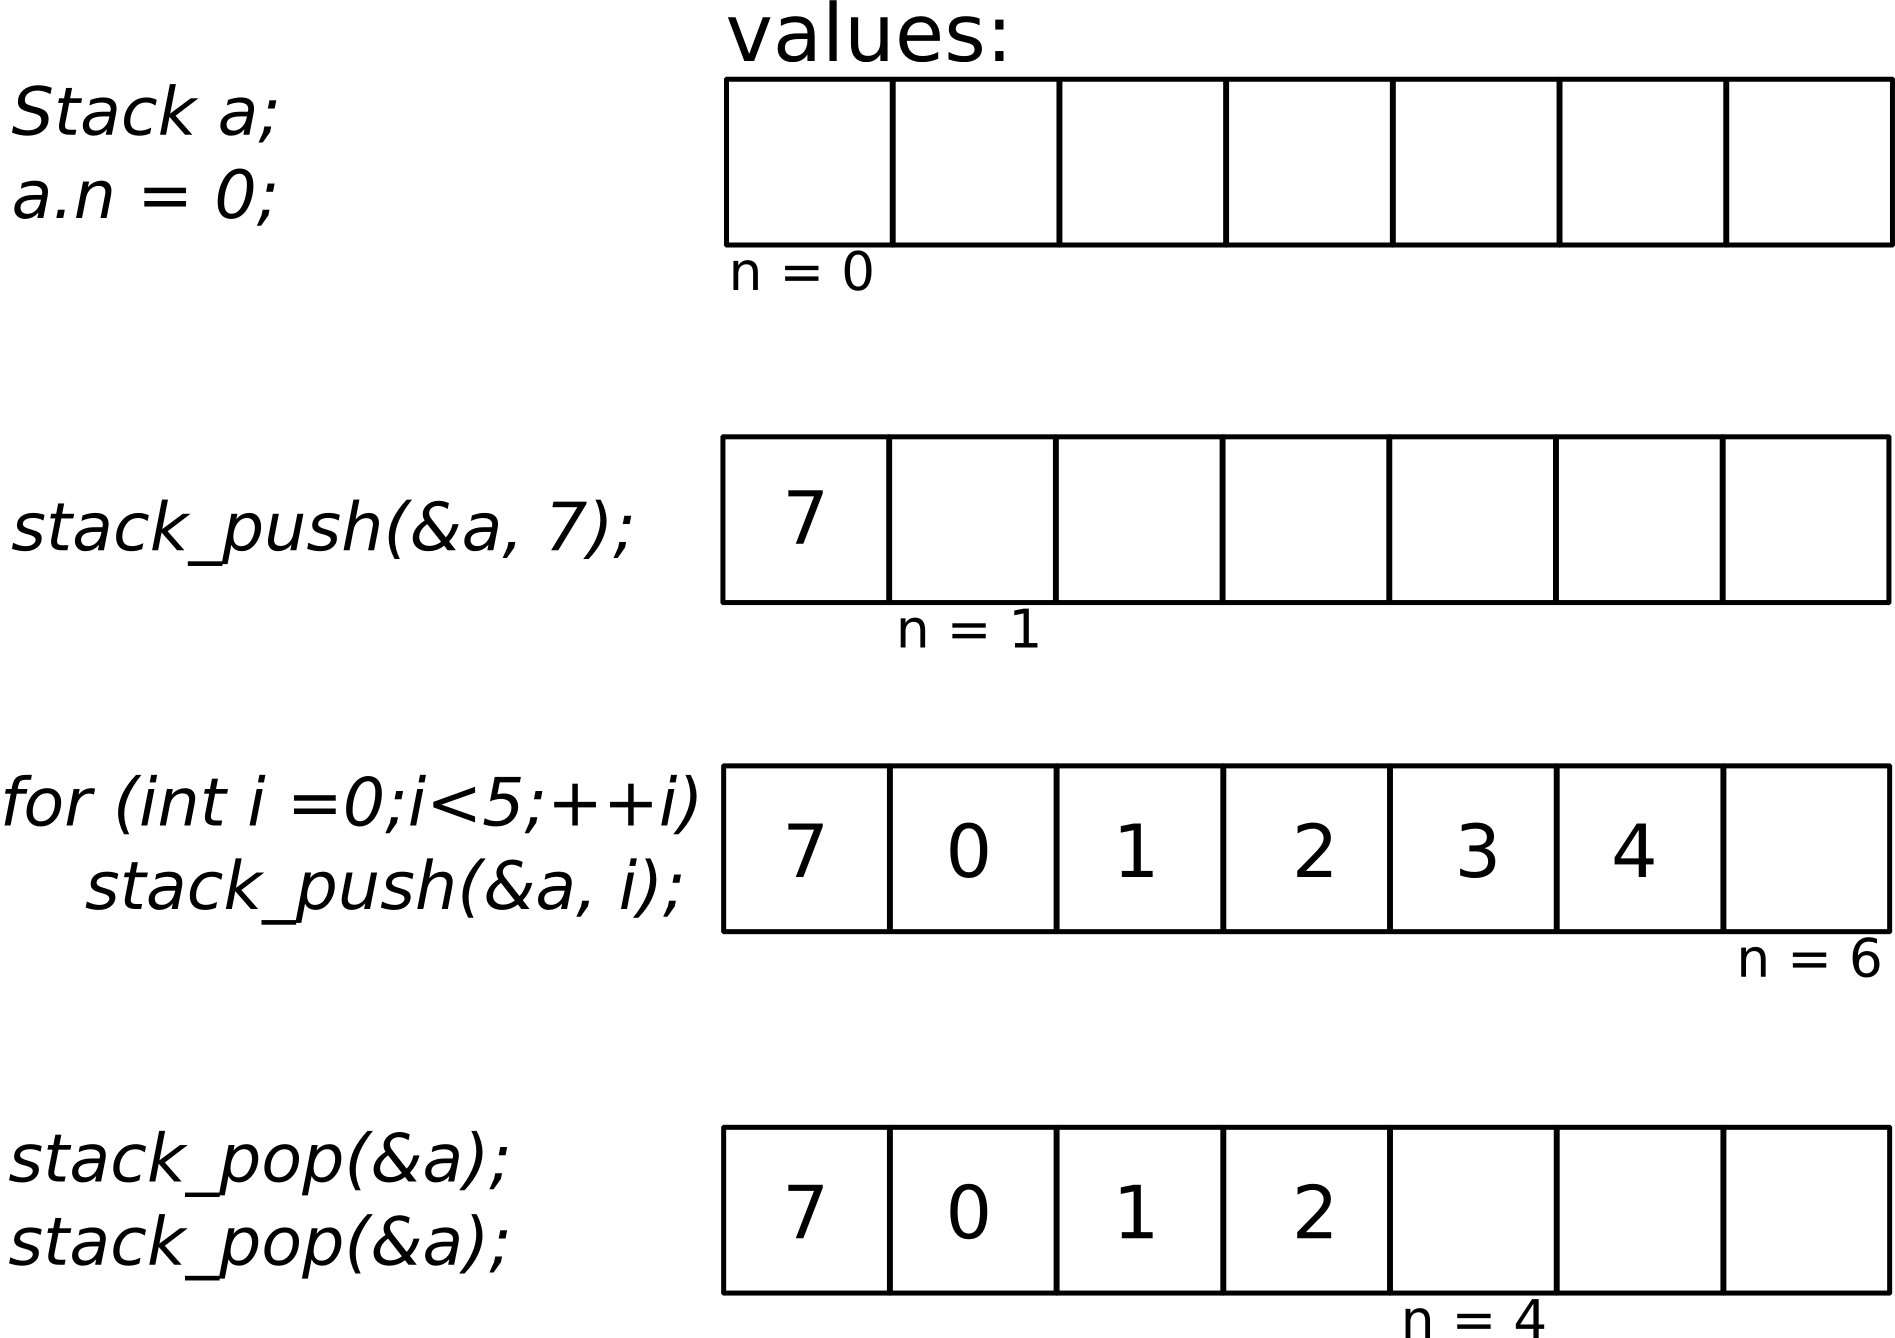
\includegraphics[width=0.95\linewidth]{../images/stack.png}
\end{center}
\end{multicols}

\subsubsection*{Задачи:}
\begin{enumerate}
\item Написать функцию \textbf{int} stack\_pop(Stack* s, \textbf{int} x). Протестируёте стек: проверьте, что выведет программа, написанная выше.
\item Написать функцию \textbf{int} stack\_is\_empty(Stack* s), которая возвращает 1 если стек пуст и 0 иначе.
\item Написать функцию \textbf{int} stack\_get(Stack* s), которая возвращает элемент, находящийся в вершине стека, но не изменяет стек.
\item Написать функцию \textbf{void} stack\_print(Stack* s), которая распечатывает все элементы стека.
\item Одна из проблем текущей реализации: размер массива 100 захардкожен. Чтобы решить эту проблему введите \#define-константу CAPACITY:
\begin{verbatim}
#define CAPACITY 100
\end{verbatim}
\item Что произойдёт, если вызвать stack\_push() при полном стеке? Обработайте эту ситуацию. Программа должна печатать сообщение об ошибке и завершаться с аварийным кодом завершения. Чтобы завершить программу таким образом можно использовать функцию exit() из библиотеки stdlib.h. Пример вызова: exit(1);
\item Аналогично при вызове stack\_pop() и stack\_get() при пустом стеке.
\item Введите функцию stack\_init(), которая будет ответственна за настройку стека сразу после его создания. В данном случае, единственное, что нужно сделать после создания стека это занулить n.
\item Предположим, что вы однажды захотите использовать стек не для целочисленных чисел типа int, а для какого-нибудь другого типа (например char). Введите синоним для типа элементов стека:
\begin{verbatim}
typedef int Data;
\end{verbatim}
Измените тип элемента стека во всех функциях с int на Data (тип поля n менять не нужно). Теперь вы в любой момент сможете изменить тип элементов стека, изменив лишь одну строчку.
\item Сложные скобки. Решить задачу определения правильной скобочной последовательности, используя стек символов. Виды скобок: () \{\} [] <>. Пример неправильной последовательности: (\{<\}>)
\item Стек с динамическим выделением памяти. Описание такого стека выглядит следующим образом:
\begin{verbatim}
struct stack
{
    int capacity;
    int n;
    Data* values;
};
typedef struct stack Stack;
\end{verbatim}
Введено новое поле capacity. В нём будет хранится количество элементов стека, под которые уже выделена память. В отличии от предыдущего варианта стека, это значение будет меняться. \\
values теперь не статический массив, а указатель. Вы должны выделить необходимое место для стека в функции stack\_init(). Начальное значение capacity можно выбрать самостоятельно либо передавать на вход функции stack\_init(). При заполнении стека должно происходить перевыделение памяти с помощью функции realloc().
\end{enumerate}


\subsubsection*{Структуры и malloc (дополнительное задание)} 
\begin{enumerate}
\item Объявить структуру, которая будет описывать замеры температуры. Она должна содержать следующие поля: 
\begin{itemize}
\item char scale -- символ, обозначающий шкалу измерений: 'C' -- градусы Целься, 'K' -- Кельвина, 'F' -- Фаренгейта.
\item double temperature -- вещественное число -- температура в этой шкале
\item int data -- целое число -- день замера температуры
\end{itemize}
\item Чему равен размер этой структуры в байтах? Найти её размер с помощью sizeof() и напечатать его на экран.
\item Создать динамический массив для хранения 50-ти таких структур.
\item Увеличить размер этого массива с 50 до 1000.
\item Освободить всю память, которую вы выделили.
\end{enumerate}
\end{document}